\documentclass[a4paper,12pt]{jsarticle}
\usepackage{amsmath,amssymb}
\usepackage{ascmac}
\usepackage{bbold}
\usepackage{bm}
\usepackage{braket}
\usepackage{cases}
\usepackage{dsfont}
\usepackage[dvipdfmx]{hyperref,graphicx}
\usepackage{pxjahyper}
\usepackage{fancyhdr}
\usepackage{feynmf}
\usepackage{here}
\usepackage{lastpage}
\usepackage{latexsym}
\usepackage{listings}
\usepackage{mathrsfs}
\usepackage{tcolorbox}

\renewcommand{\lstlistingname}{ソースコード}

\makeatletter
\@addtoreset{equation}{section}
\def\theequation{\thesection.\arabic{equation}}
\makeatother

\lstset{
  basicstyle={\ttfamily},
  identifierstyle={\small},
  commentstyle={\smallitshape},
  keywordstyle={\small\bfseries},
  ndkeywordstyle={\small},
  stringstyle={\small\ttfamily},
  frame={tb},
  breaklines=true,
  columns=[l]{fullflexible},
  numbers=left,
  xrightmargin=0zw,
  xleftmargin=3zw,
  numberstyle={\scriptsize},
  stepnumber=1,
  numbersep=1zw,
  lineskip=-0.5ex
}

\title{\LaTeX 入門}
\author{秋山進一郎\\筑波大学計算科学研究センター}
\date{\today}

\begin{document}

\maketitle

\section{\LaTeX による文書作成にあたって}

まず, 新しい文書を作成するごとにそれ専用のディレクトリを準備する.
文書の名前はディレクトリ名で管理する.
以下では,このディレクトリをメインディレクトリと呼ぶ.
まずはメインディレクトリの中に.texファイルを作成する.
文章に掲載する図は画像ファイルとしてメインディレクトリに格納する.
図は全てベクターファイルで格納する.
ベクターファイルを使う理由は,図の拡大,縮小時に解像度が低下しないためである.
代表的なベクターファイルは.pdf, .epsなどである.
\footnote{
ピクセルで構成されているラスターファイル(.jpeg, .pngなど)の使用は避ける.
}
引用文献はBibTeXで管理することとし, .bibファイルを作成する.
この.bibファイルもメインディレクトリに格納する.

ここでは, 親となる.texファイルにはmain.texと名前を付けることにする.
例えば, Overleafでもデフォルトの.texファイル名はmain.texである.
画像ファイルはfigという名前のディレクトリを作ってそこに格納する.
同様に, bibファイルはbibという名前のディレクトリを作って格納する.
例えば, 卒業論文を作成する場合なら,senior$\_$thesisという名前のメインディレクトリを作成し, その中にmain.texを作成する.
そして, senior$\_$thesisディレクトリの中にfigディレクトリとbibディレクトリを作成する.
実験や数値計算の結果をまとめた画像ファイルは全てfigディレクトリに格納する.
参考文献や引用文献の情報は全て.bibファイルで管理し, bibディレクトリに格納する.

なお,Overleafで日本語入力ができるようにするためには,メインディレクトリにlatexmkrcという名前のファイルを作成し,以下の内容をlatexmkrcにコピーしておく必要がある.
その後,左上の「Menu」から「Compiler」へ行き,「pdfLaTeX」を「LaTeX」に変更する.
\begin{lstlisting}[caption=latexmkrc]
    $latex = 'uplatex';
    $bibtex = 'upbibtex';
    $dvipdf = 'dvipdfmx %O -o %D %S';
    $makeindex = 'mendex -U %O -o %D %S';
    $pdf_mode = 3; 
\end{lstlisting}

\section{パッケージ}

パッケージを指定することにより,様々な数学表現,物理学の記法,書体などが\LaTeX で使用可能になる.
パッケージを指定するには,\texttt{\textbackslash usepackage\{パッケージ名\}}をプリアンブル(Preamble)に書けば良い.
プリアンブルとは,.texファイルの冒頭から\texttt{\textbackslash begin$\{$document$\}$}までのことを言う.
ソースコード\ref{sample}の1行目と4行目の間がプリアンブルである.

\begin{lstlisting}[caption=.texファイルで基本となる構造,label=sample]
    \documentclass[a4paper,12pt]{jsarticle}
    % Preamble
    
    \begin{document}
    % Main text
    
    \end{document}
\end{lstlisting}


これから自分が作成する文書において,どのようなパッケージが必要になるかを予め把握しようとするのは得策ではない.
文書作成を進める中で「こういう数学表現を使いたいが,\LaTeX ではどのように書くのだろう?」というニーズが発生した際に,その都度調べる方が良い.
アメリカ数学会(American Mathematical Society; AMS)がサポートしている\texttt{amsmath}パッケージは物理の分野でも重宝されている.
同じ数学表現であっても,異なるパッケージで異なる記述方法が与えられていることも多々ある.
各自で自分好みの使いやすいものを見つけていってもらいたい.
\footnote{
時たま,パッケージの組み合わせに起因してコンパイルが出来ないことがある(パッケージAとパッケージBを同時に指定するとエラーになる,パッケージBを指定する場合にはパッケージAよりも先に指定しなければならない,など).
そういうこともあるのだと頭の片隅に入れておくとどこかで役に立つかもしれない.
}
\footnote{
例えば,以下のサイトでは数学記号や特殊文字を手書き入力すると,\LaTeX でそれを再現するために必要なパッケージと使い方が検索される.
\url{https://detexify.kirelabs.org/classify.html}
}

\section{環境}

\LaTeX における環境とは,\texttt{\textbackslash begin$\{*\}$}と\texttt{\textbackslash end$\{*\}$}という対で囲まれた部分のことを指す.
どういう環境かを呼称するために,$\{*\}$の部分を使って,「$*$環境」と言うことがある.
例えば,多くの.texファイルでは,プリアンブルの直後は\texttt{document}環境になっている.
ソースコード\ref{sample}で言えば,4行目と7行目の間に文章や数式を入力していくことになる.
数式を書く場合には,数式環境を用意する必要がある.
代表的な数式環境として,\texttt{equation}環境,\texttt{eqnarray}環境,\texttt{align}環境などがある.
例えば,\texttt{align}環境を使う場合は下のようになる.
\begin{lstlisting}[caption=\texttt{align}環境による記述]
    \begin{align}
    % Equation
    \end{align}
\end{lstlisting}

\section{文書入力のルール}

文書の表題には,表題,著者名,著者の所属,作成日時を書く.
これらはプリアンブルで,\texttt{\textbackslash title$\{$表題$\}$},\texttt{\textbackslash author$\{$著者名\textbackslash\textbackslash 著者の所属$\}$},\texttt{\textbackslash date$\{$\textbackslash today$\}$}を記述し,\texttt{\textbackslash begin$\{$document$\}$}のすぐ下で\texttt{\textbackslash maketitle}を書くことで出力される.
\footnote{論文の場合には要旨も書く.}
下のソースコードを参照せよ.
\begin{lstlisting}[caption=表題の作成,label=title]
    \documentclass[a4paper,12pt]{jsarticle}
    % Preamble
    \title{Title}
    \author{Name\\Institution}
    \date{\today}

    \begin{document}
    \maketitle
    % Main text
    \end{document}
\end{lstlisting}

通常の文章は\texttt{\textbackslash maketitle}の下に記述していく.
\LaTeX では,\texttt{\%}で始まる行はコメントと見なされ,コンパイルしても出力されない.
これをコメントアウトと呼ぶ.
行の途中に\texttt{\%}を書いた場合,そこからその行の最後までがコメントアウトされる.
.texファイル(以下ではソースファイルとも呼ぶ)に入力した文章は,それが最も美しく清書されるように\LaTeX が自動的に改行を入れてくれる.
ソースファイル上で改行を行っても出力される清書には改行が反映されない.
指定した場所に改行を施したい場合は,ソースファイル上で\textbackslash\textbackslash を入れる必要がある.
また,空行を入れると改段落される.
\footnote{
改ページしたい場合は,改ページしたい場所で\texttt{\textbackslash clearpage}と書けばよい.
}
章や節のタイトルは,\texttt{\textbackslash chapter$\{\}$},\texttt{\textbackslash section$\{\}$},\texttt{\textbackslash subsection$\{\}$}などで指定できる.
章や節の番号は\LaTeX が自動で割り振ってくれる.
\footnote{
これらの番号を自分で変更したい場合には,\texttt{\textbackslash setcounter$\{\}$}を使う.
}
箇条書きをする場合,\texttt{itemize}環境や\texttt{enumerate}環境を使うと良い.
以下は,\texttt{itemize}環境による記述である.
\begin{lstlisting}[caption=\texttt{itemize}環境による記述]
    \begin{itemize}
        \item \texttt{itemize}環境を使う
        \item \texttt{itemize}環境を使う
        \item \texttt{itemize}環境を使う
    \end{itemize}
\end{lstlisting}
\begin{itemize}
    \item \texttt{itemize}環境を使う
    \item \texttt{itemize}環境を使う
    \item \texttt{itemize}環境を使う
\end{itemize}
以下は,\texttt{enumerate}環境による記述である.
こちらの環境では連番が付される.
\begin{lstlisting}[caption=\texttt{enumerate}環境による記述]
    \begin{enumerate}
        \item \texttt{enumerate}環境を使う
        \item \texttt{enumerate}環境を使う
        \item \texttt{enumerate}環境を使う
    \end{enumerate}
\end{lstlisting}
\begin{enumerate}
    \item \texttt{enumerate}環境を使う
    \item \texttt{enumerate}環境を使う
    \item \texttt{enumerate}環境を使う
\end{enumerate}
いずれの環境でも,\texttt{\textbackslash item}によって新しい箇条書きの項目を開始する.

\section{表の作成}

表の作成には,\texttt{table}環境と\texttt{tabular}環境を使う.
具体例として,表\ref{tab:sample}とそのソースコード\ref{table_sample}を見よ.
\texttt{\textbackslash hline}によって横線が一本引かれる.
\texttt{\textbackslash hline \textbackslash hline}と書けば二重の横線を引くことができる.
表の各行において,それぞれの要素の間は\texttt{\&}で区切る.
行の最後には\texttt{\textbackslash \textbackslash}を書く.
表\ref{tab:sample}では,各行が四つの要素から構成されている.
そして,各要素は中央揃えで表示されている.
これは,ソースファイル上の\texttt{\textbackslash begin$\{$tabular$\}$$\{$c|c|c|c$\}$}の部分で制御されている.
\texttt{$\{$c|c|c|c$\}$}の\texttt{|}によって縦線が出力される.\texttt{|}を消すと縦線が消えた表になる.
また,\texttt{c}を\texttt{l},\texttt{r}に変更すると,左揃え,右揃えに変えることができる.
表に対するキャプションは\texttt{\textbackslash caption$\{\}$}で記述する.
\begin{lstlisting}[caption=表\ref{tab:sample},label=table_sample]
    \begin{table}[H]
        \centering
        \caption{Gauge boson}
        \begin{tabular}{c|c|c|c}
            \hline
            Name & Mass (GeV) & Electronic charge & Interaction \\
            \hline\hline
            Photon & $0$ & $0$ & Electromagnetic \\ 
            Gluon & $0$ & $0$ & Strong \\ 
            $W$ boson & $89.3$ & $\pm1$ & Electromagnetic, Weak, Gravity \\ 
            $Z$ boson & $93$ & $0$ & Weak, Gravity \\ 
            Graviton & $0$ & $0$ & Gravity \\ 
            \hline
        \end{tabular}
        \label{tab:sample}
    \end{table}
\end{lstlisting}

\begin{table}[H]
    \centering
    \caption{Gauge boson}
    \begin{tabular}{c|c|c|c}
        \hline
        Name & Mass (GeV) & Electronic charge & Interaction \\
        \hline\hline
        Photon & $0$ & $0$ & Electromagnetic \\ 
        Gluon & $0$ & $0$ & Strong \\ 
        $W$ boson & $89.3$ & $\pm1$ & Electromagnetic, Weak, Gravity \\ 
        $Z$ boson & $93$ & $0$ & Weak, Gravity \\ 
        Graviton & $0$ & $0$ & Gravity \\ 
        \hline
    \end{tabular}
    \label{tab:sample}
\end{table}

\section{図の挿入}

まずはgnuplotやPythonで作成した図(.pdfや.eps)をfigディレクトリに格納する.
例として,figディレクトリに格納したsample.pdfを文章中に挿入する.
ソースファイル上で\texttt{fig}環境を作り,その中で\texttt{\textbackslash includegraphics$\{$fig/sample.pdf$\}$}と書けば図を挿入できる(図\ref{fig:sample}).
表の場合と同様,図の説明を\texttt{\textbackslash caption$\{\}$}で記述できる.
実際のソースコードでは,\texttt{\textbackslash includegraphics[scale=1]$\{$fig/sample.pdf$\}$}となっているが,\texttt{[scale=1]}は図の大きさを調整するためのオプションである.
\LaTeX では,図を表示する場所が自動的に調整されるが,\texttt{\textbackslash begin$\{$figure$\}$}にオプションを付すことで,その場所を自分で操作することもできる.
例えば,\texttt{\textbackslash begin$\{$figure$\}$[h]}とすると,ソースファイル上で\texttt{\textbackslash includegraphics}したその場所に図を優先的に表示させることができる.
\footnote{
その場所に強制的に表示させたい場合は,\texttt{here.sty}を使い,\texttt{\textbackslash usepackage$\{$here$\}$}をプリアンブルに書いた上で,\texttt{\textbackslash begin$\{$figure$\}$[H]}とする.
}
\begin{lstlisting}[caption=図\ref{fig:sample}]
    \begin{figure}
        \centering
        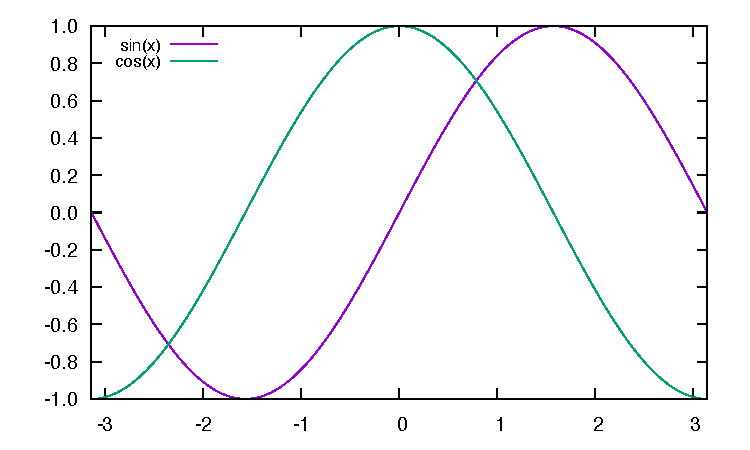
\includegraphics[scale=1]{fig/sample.pdf}
        \caption{Trigonometric functions}
        \label{fig:sample}
    \end{figure}
\end{lstlisting}

\begin{figure}[H]
    \centering
    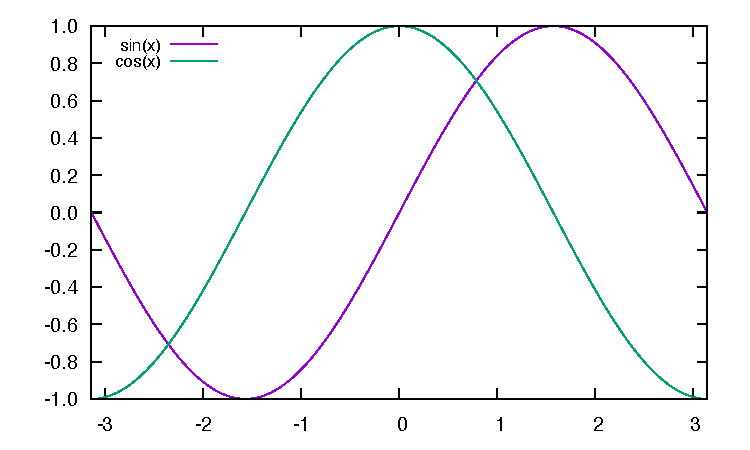
\includegraphics[scale=1]{fig/sample.pdf}
    \caption{Trigonometric functions}
    \label{fig:sample}
\end{figure}

\section{数式,図,表の参照}

\LaTeX では,数式,図,表には番号が自動的に割り振られ,\texttt{\textbackslash label$\{*\}$}と\texttt{\textbackslash ref$\{*\}$}のペアでこれらの番号を容易に参照することができる.
ここで,\texttt{\textbackslash label$\{*\}$}と\texttt{\textbackslash ref$\{*\}$}のペアにおいて,\texttt{$\{*\}$}には自分の好きな名前を与えることができるが,数式に対しては\texttt{$\{$eq:*$\}$},表に対しては\texttt{$\{$tab:*$\}$},図に対しては\texttt{$\{$fig:*$\}$},のように参照名をつけるのが慣習である.
例えば,数式を式番号で参照する場合,参照したい数式が記述されている環境内に\texttt{\textbackslash label$\{$eq:*$\}$}を書いておく.
そして,文章中で\texttt{\textbackslash ref$\{$eq:*$\}$}と書けばその式番号が表示される.
実際には,式番号には丸括弧()を付けることが多いため,\texttt{ (\textbackslash ref$\{$eq:*$\}$)}とするか,数式専用の参照方法として\texttt{\textbackslash eqref$\{$eq:*$\}$}を用いることが多い.
実際に以下の数式を参照してみると次のようになる.
\begin{lstlisting}[caption=式\eqref{eq:sample}]
    \begin{align}
        \label{eq:sample}
        f(x)=x
    \end{align}
\end{lstlisting}
\begin{align}
\label{eq:sample}
    f(x)=x
\end{align}
上の式は式\eqref{eq:sample}として参照される.
この式よりも前に別の式を書き足しても,\LaTeX が勝手に新しい式番号をつけ,\texttt{\textbackslash label$\{*\}$}と\texttt{\textbackslash ref$\{*\}$}によって新しい式番号が参照される.
式番号そのものをソースファイル上で打つ(ハードコーディング)のは避ける.
ハードコーディングは間違いの元である.
また,異なる式には異なる参照名を与えること.

\section{いくつかの数学表現}

\subsection{諸注意と数学関数}

数式を書くためには数式環境を使う.
例えば,\texttt{align}環境を使う場合,\texttt{\textbackslash begin$\{$align$\}$}と\texttt{\textbackslash end$\{$align$\}$}の間に数式を入力していく.
もし,文章中で数式を書く場合には\texttt{\$}で数式を挟む必要がある.
\footnote{インライン数式モードなどと呼ばれる.}

数式環境では,文字はすべて斜体で表示される.
例えば,ソースファイル上で\texttt{\$sin x\$}と書くと,$sin x$となる.
このような数学関数は斜体ではなく,立体で表示するのがルールである.
多くの数学関数は,\texttt{\textbackslash}に数学関数の名前を続けると立体で表示される.
今の場合,\texttt{\$\textbackslash sin x\$}とすれば,$\sin x$と出力される.
注意すべきは,\texttt{\textbackslash sin x}のように\texttt{\textbackslash sin}と\texttt{x}の間にはスペースが必要なことである.
スペースなしで\texttt{\textbackslash sinx}と書いてしまうと,\texttt{\textbackslash sinx}というコマンドとして見なされる.
指定しているパッケージ内に存在しないコマンドを入力してしまうと当然エラーになる.
主な数学関数を表\ref{tab:math}に示す.
\begin{table}[H]
    \centering
    \caption{主な数学関数}
    \begin{tabular}{lc|lc|lc}
        \hline
        コマンド & 出力 & コマンド & 出力 & コマンド & 出力\\
        \hline\hline
        \texttt{\textbackslash cos} & $\cos$ & \texttt{\textbackslash sin} & $\sin$ & \texttt{\textbackslash tan} & $\tan$ \\ 
        \texttt{\textbackslash cosh} & $\cosh$ & \texttt{\textbackslash sinh} & $\sinh$ & \texttt{\textbackslash tanh} & $\tanh$ \\ 
        \texttt{\textbackslash exp} & $\exp$ & \texttt{\textbackslash ln} & $\ln$ & \texttt{\textbackslash log} & $\log$ \\ 
        \texttt{\textbackslash sec} & $\sec$ &
        \texttt{\textbackslash csc} & $\csc$ &  \texttt{\textbackslash cot} & $\cot$ \\ 
        \texttt{\textbackslash lim} & $\lim$ & \texttt{\textbackslash sup} & $\sup$ & \texttt{\textbackslash inf} & $\inf$ \\ 
        \hline
    \end{tabular}
    \label{tab:math}
\end{table}

なお,物理の分野では,物理的に意味のある量は斜体で記述するが,物理的な意味を持たない定数などは立体で書くというルールがある.例えば,素電荷はよく$e$で表すのに対し,Napier数は${\rm e}$と表記する.
数式環境でアルファベットを立体にするには,\texttt{\textbackslash mathrm$\{$アルファベット$\}$}とすれば良い.
他にも,虚数単位は$\mathrm{i}$のように立体で書く.
微分記号の$\mathrm{d}$も立体で書く.
例えば,指数関数$\mathrm{e}^{x}$の微分は,

\begin{lstlisting}[caption=式\eqref{eq:dx_exp},label=dx_exp]
    \begin{align}
        \frac{\mathrm{d}}{\mathrm{d}x}\mathrm{e}^{x}
        = \mathrm{e}^{x}
    \end{align}
\end{lstlisting}
\begin{align}
\label{eq:dx_exp}
    \frac{\mathrm{d}}{\mathrm{d}x}\mathrm{e}^{x}
    =
    \mathrm{e}^{x}
\end{align}
のように書く.
なお,ソースコード\ref{dx_exp}では見やすさを優先してインデントや改行が入っているが,これらがなくても式\eqref{eq:dx_exp}と同じ出力が得られる.
実際,以下のように書いても全く問題ない.
\begin{lstlisting}[caption=式\eqref{eq:dx_exp}]
    \begin{align}
    \frac{\mathrm{d}}{\mathrm{d}x}\mathrm{e}^{x}=\mathrm{e}^{x}
    \end{align}
\end{lstlisting}
以下のソースコードでは,常に見やすさを優先してインデントや改行が適宜入れてある.

\subsection{ギリシャ文字}

ギリシャ文字は大変よく使う.
表\ref{tab:greek}がギリシャ文字の一覧である.
大文字にするには,コマンドの頭文字だけ大文字にする.
例えば,$\Psi$を表示するためには\texttt{\textbackslash Psi}と書く.
ただし,全てのギリシャ文字がこのルールに従っているわけではなく,通常のアルファベットの大文字で代用する場合もある.
例えば,$\alpha$の大文字は$A$であり,これは単に\texttt{A}と打つだけで良い.
また,いくつかのギリシャ文字については,綴りの前に\texttt{var}を付けることで書体の変更が可能である.
例えば,単に\texttt{\textbackslash epsilon}と書くと$\epsilon$となるが,\texttt{\textbackslash varepsilon}と書くと$\varepsilon$になる.
\begin{table}[H]
    \centering
    \caption{ギリシャ文字}
    \begin{tabular}{lc|lc|lc}
        \hline
        コマンド & 出力 & コマンド & 出力 & コマンド & 出力\\
        \hline\hline
        \texttt{\textbackslash alpha} & $\alpha$ & \texttt{\textbackslash iota} & $\iota$ & \texttt{\textbackslash rho} & $\rho$ \\ 
        \texttt{\textbackslash beta} & $\beta$ & \texttt{\textbackslash kappa} & $\kappa$ & \texttt{\textbackslash sigma} & $\sigma$ \\ 
        \texttt{\textbackslash gamma} & $\gamma$ & \texttt{\textbackslash lambda} & $\lambda$ & \texttt{\textbackslash tau} & $\tau$ \\ 
        \texttt{\textbackslash delta} & $\delta$ & \texttt{\textbackslash mu} & $\mu$ & \texttt{\textbackslash upsilon} & $\upsilon$ \\ 
        \texttt{\textbackslash epsilon} & $\epsilon$ & \texttt{\textbackslash nu} & $\nu$ & \texttt{\textbackslash phi} & $\phi$ \\ 
        \texttt{\textbackslash zeta} & $\zeta$ & \texttt{\textbackslash xi} & $\xi$ & \texttt{\textbackslash chi} & $\chi$ \\ 
        \texttt{\textbackslash eta} & $\eta$ & \texttt{o} & $o$ & \texttt{\textbackslash psi} & $\psi$ \\ 
        \texttt{\textbackslash theta} & $\theta$ & \texttt{\textbackslash pi} & $\pi$ & \texttt{\textbackslash omega} & $\omega$ \\ 
        \hline
    \end{tabular}
    \label{tab:greek}
\end{table}

\subsection{数学記号,特殊文字}

数式環境の中で使うことのできる数学記号,特殊文字のいくつかを表\ref{tab:symbol}に示す.


\begin{table}[H]
    \centering
    \caption{代表的な数学記号,特殊文字}
    \begin{tabular}{lc|lc}
        \hline
        コマンド & 出力 & コマンド & 出力 \\
        \hline\hline
        \texttt{\textbackslash equiv} & $\equiv$  & 
        \texttt{\textbackslash approx} & $\approx$  \\
        \texttt{\textbackslash simeq} & $\simeq$  & 
        \texttt{\textbackslash sim} & $\sim$  \\ 
        \texttt{\textbackslash le} & $\le$  &
        \texttt{\textbackslash ge} & $\ge$  \\
        \texttt{\textbackslash lesssim} & $\lesssim$  &
        \texttt{\textbackslash gtrsim} & $\gtrsim$  \\ 
        \texttt{\textbackslash to} & $\to$ &
        \texttt{\textbackslash mapsto} & $\mapsto$  \\ 
        \texttt{\textbackslash rightarrow} & $\rightarrow$ &
        \texttt{\textbackslash Rightarrow} & $\Rightarrow$ \\
        \texttt{\textbackslash leftarrow} & $\leftarrow$ &
        \texttt{\textbackslash Leftarrow} & $\Leftarrow$ \\
        \texttt{\textbackslash leftrightarrow} & $\leftrightarrow$ &
        \texttt{\textbackslash Leftrightarrow} & $\Leftrightarrow$ \\
        \texttt{\textbackslash pm} & $\pm$  &
        \texttt{\textbackslash mp} & $\mp$  \\
        \texttt{\textbackslash propto} & $\propto$  &
        \texttt{\textbackslash infty} & $\infty$  \\
        \texttt{\textbackslash times} & $\times$  &
        \texttt{\textbackslash otimes} & $\otimes$  \\
        \texttt{\textbackslash partial} & $\partial$  & 
        \texttt{\textbackslash nabla} & $\nabla$  \\
        \texttt{\textbackslash dagger} & $\dagger$  & 
        \texttt{\textbackslash hbar} & $\hbar$  \\
        \texttt{\textbackslash cdot} & $\cdot$  &
        \texttt{\textbackslash cdots} & $\cdots$  \\
        \hline
    \end{tabular}
    \label{tab:symbol}
\end{table}



\subsection{添え字}

上付きの添え字を書くためには\texttt{$\hat{}$}を使う.
下付きの添え字には\texttt{$\_{}$}を使う.

\begin{lstlisting}[caption=式\eqref{eq:2_2024}]
    \begin{align}
        2^{2024}
    \end{align}
\end{lstlisting}
\begin{align}
\label{eq:2_2024}
    2^{2024}
\end{align}

\begin{lstlisting}[caption=式\eqref{eq:a1}]
    \begin{align}
        a_{1},a_{2},a_{3}
    \end{align}
\end{lstlisting}
\begin{align}
\label{eq:a1}
    a_{1},a_{2},a_{3}
\end{align}

上付き,下付きの添え字を組み合わせる場合はどちらを先に書いても構わない.
\begin{lstlisting}[caption=式\eqref{eq:tensor}]
    \begin{align}
        g^{\mu}_{\nu}, g_{\nu}^{\mu}
    \end{align}
\end{lstlisting}
\begin{align}
\label{eq:tensor}
    g^{\mu}_{\nu}, g_{\nu}^{\mu}
\end{align}

なお,ソースコード上で上付き,下付きの添え字は必ずしも\texttt{$\{\}$}で括る必要はないが,次の例から注意が必要なことが分かるだろう.
\begin{lstlisting}[caption=式\eqref{eq:tensor_remark}]
    \begin{align}
        g^{\mu\nu}, g^\mu\nu
    \end{align}
\end{lstlisting}
\begin{align}
\label{eq:tensor_remark}
    g^{\mu\nu}, g^\mu\nu
\end{align}

\subsection{分数}

分数は\texttt{\textbackslash frac$\{$分子$\}$$\{$分母$\}$}と書く.

\begin{lstlisting}[caption=式\eqref{eq:tanx}]
    \begin{align}
        \tan x = \frac{\sin x}{\cos x}
    \end{align}
\end{lstlisting}
\begin{align}
\label{eq:tanx}
    \tan x=\frac{\sin x}{\cos x}
\end{align}

\subsection{大型演算子}

和は\texttt{\textbackslash sum},積は\texttt{\textbackslash prod},積分は\texttt{\textbackslash int}で書く.
これらの上端,下端は上付き,下付き添え字で書く.
\begin{lstlisting}[caption=式\eqref{eq:sum}]
    \begin{align}
        \sum_{k=1}^{\infty}\frac{1}{k^{2}}
        = \frac{\pi^2}{6}
    \end{align}
\end{lstlisting}
\begin{align}
\label{eq:sum}
    \sum_{k=1}^{\infty}
    \frac{1}{k^{2}}
    =
    \frac{\pi^2}{6}
\end{align}

\begin{lstlisting}[caption=式\eqref{eq:prod}]
    \begin{align}
        \prod_{k=1}^{\infty}\frac{(2k)^{2}}{(2k-1)(2k+1)}
        = \frac{\pi}{2}
    \end{align}
\end{lstlisting}
\begin{align}
\label{eq:prod}
    \prod_{k=1}^{\infty}
    \frac{(2k)^{2}}{(2k-1)(2k+1)}
    =
    \frac{\pi}{2}
\end{align}

\begin{lstlisting}[caption=式\eqref{eq:int}]
    \begin{align}
        \int^{2\pi}_{0}\mathrm{d}x\cos x
        = 0
    \end{align}
\end{lstlisting}
\begin{align}
\label{eq:int}
    \int^{2\pi}_{0}
    \mathrm{d}x\cos x
    =
    0
\end{align}

\subsection{根号}

根号は\texttt{\textbackslash sqrt$\{\}$}で書く.
$n$乗根の場合は\texttt{\textbackslash sqrt[n]$\{\}$}と書く.
\begin{lstlisting}[caption=式\eqref{eq:sqrt}]
    \begin{align}
        \sqrt{1+x}
    \end{align}
\end{lstlisting}
\begin{align}
\label{eq:sqrt}
    \sqrt{1+x}
\end{align}

\begin{lstlisting}[caption=式\eqref{eq:sqrt_n}]
    \begin{align}
        \sqrt[4]{1+x}
    \end{align}
\end{lstlisting}
\begin{align}
\label{eq:sqrt_n}
    \sqrt[4]{1+x}
\end{align}

\subsection{ベクトル}

ベクトルは太文字を使う.
太文字にするには,\texttt{bm}パッケージを指定した上で\texttt{\textbackslash bm$\{\}$}を使う.

\begin{lstlisting}[caption=式\eqref{eq:bm}]
    \begin{align}
        \bm{x}
    \end{align}
\end{lstlisting}
\begin{align}
\label{eq:bm}
    \bm{x}
\end{align}
もし矢印でベクトルを表したい場合は\texttt{\textbackslash vec$\{\}$}を使う.

\begin{lstlisting}[caption=式\eqref{eq:vec}]
    \begin{align}
        \vec{x}
    \end{align}
\end{lstlisting}
\begin{align}
\label{eq:vec}
    \vec{x}
\end{align}

ベクトルの成分をあらわに書く場合は,\texttt{pmatrix}環境を使うと良い.
数式環境の中に\texttt{pmatrix}環境を作ることに注意.

\begin{lstlisting}[caption=式\eqref{eq:vec_pmatrix}]
    \begin{align}
        \bm{x} =
        \begin{pmatrix}
            x_{1} \\
            x_{2} \\
            x_{3}
        \end{pmatrix}
    \end{align}
\end{lstlisting}
\begin{align}
\label{eq:vec_pmatrix}
    \bm{x}
    =
    \begin{pmatrix}
        x_{1} \\
        x_{2} \\
        x_{3}
    \end{pmatrix}
\end{align}
また,\texttt{bmatrix}環境を使うと,

\begin{lstlisting}[caption=式\eqref{eq:vec_bmatrix}]
    \begin{align}
        \bm{x} =
        \begin{bmatrix}
            x_{1} \\
            x_{2} \\
            x_{3}
        \end{bmatrix}
    \end{align}
\end{lstlisting}
\begin{align}
\label{eq:vec_bmatrix}
    \bm{x}
    =
    \begin{bmatrix}
        x_{1} \\
        x_{2} \\
        x_{3}
    \end{bmatrix}
\end{align}
となる.

\subsection{文字装飾}

アルファベットに対する装飾をいくつか紹介する.
ハット記号は\texttt{\textbackslash hat$\{\}$},チルダ記号は\texttt{\textbackslash tilde$\{\}$},ドット記号は\texttt{\textbackslash dot$\{\}$}を使う.

\begin{lstlisting}[caption=式\eqref{eq:hat}]
    \begin{align}
        \hat{H},~\tilde{I},~\dot{J}
    \end{align}
\end{lstlisting}
\begin{align}
\label{eq:hat}
    \hat{H},~\tilde{I},~\dot{J}
\end{align}
なお,ソースコード2行目で使われている$\tilde{}$はスペースを表す.

物理の分野では,ドット記号で時間微分を表す.
\begin{lstlisting}[caption=式\eqref{eq:dot}]
    \begin{align}
        \dot{x} = \frac{\mathrm{d}}{\mathrm{d}t}x
    \end{align}
\end{lstlisting}
\begin{align}
\label{eq:dot}
    \dot{x}
    =
    \frac{\mathrm{d}}{\mathrm{d}t}x
\end{align}



\subsection{行列}

すでにベクトルのところで使ったが,行列を書く場合にも\texttt{pmatrix}環境を使うと良い.
数式環境の中に\texttt{pmatrix}環境を作ることに注意.
表の作成方法と類似している.
\begin{lstlisting}[caption=式\eqref{eq:pmatrix}]
    \begin{align}
        A =
        \begin{pmatrix}
            a_{11} & a_{12} \\
            a_{21} & a_{22} 
        \end{pmatrix}
    \end{align}
\end{lstlisting}
\begin{align}
\label{eq:pmatrix}
    A
    =
    \begin{pmatrix}
        a_{11} & a_{12} \\
        a_{21} & a_{22} 
    \end{pmatrix}
\end{align}
また,\texttt{bmatrix}環境を使うと,
\begin{align}
    A
    =
    \begin{bmatrix}
        a_{11} & a_{12} \\
        a_{21} & a_{22} 
    \end{bmatrix}
\end{align}
となる.
行列式の場合は\texttt{vmatrix}環境を使うと良い.
\begin{align}
    A
    =
    \begin{vmatrix}
        a_{11} & a_{12} \\
        a_{21} & a_{22} 
    \end{vmatrix}
\end{align}
\texttt{Vmatrix}環境にすると,
\begin{align}
    A
    =
    \begin{Vmatrix}
        a_{11} & a_{12} \\
        a_{21} & a_{22} 
    \end{Vmatrix}
\end{align}
となる.

\subsection{括弧の大きさ}

以下の数式を見てみよう.
\begin{lstlisting}[caption=式\eqref{eq:small_pr}]
    \begin{align}
        \int^{n}_{0}\mathrm{d}x(1-\frac{x}{n})^{n}x^{z-1}
    \end{align}
\end{lstlisting}
\begin{align}
\label{eq:small_pr}
    \int^{n}_{0}
    \mathrm{d}x
    (1-\frac{x}{n})^{n}
    x^{z-1}
\end{align}
ここで,ソースコード4行目の丸括弧を表す\texttt{($~$)}のペアを
\texttt{\textbackslash left( \textbackslash right)}に置き換えると,丸括弧の中身に応じて丸括弧の大きさを自動的に調整してくれる.
\begin{lstlisting}[caption=式\eqref{eq:large_pr}]
    \begin{align}
        \int^{n}_{0}\mathrm{d}x\left(1-\frac{x}{n}\right)^{n}x^{z-1}
    \end{align}
\end{lstlisting}
\begin{align}
\label{eq:large_pr}
    \int^{n}_{0}
    \mathrm{d}x
    \left(1-\frac{x}{n}\right)^{n}
    x^{z-1}
\end{align}
丸括弧に限らず,\texttt{$\{~\}$}や\texttt{$[~]$}についても\texttt{\textbackslash left}と\texttt{\textbackslash right}を付すことでその大きさが自動的に調整される.
\begin{lstlisting}[caption=式\eqref{eq:prs}]
    \begin{align}
        \left[
            \left\{
                \left(
                    \frac{1}{x}
                \right)
            \right\}
        \right]
    \end{align}
\end{lstlisting}
\begin{align}
\label{eq:prs}
    \left[
        \left\{
            \left(
                \frac{1}{x}
            \right)
        \right\}
    \right]
\end{align}

\subsection{Diracのブラケット記法}

\LaTeX でDiracのブラケット記法を使う方法はいくつか考えられる.
ここでは,\texttt{braket}パッケージを使う方法を紹介する.
\texttt{braket}パッケージでは,\texttt{\textbackslash braket$\{\}$},\texttt{\textbackslash bra$\{\}$},\texttt{\textbackslash ket$\{\}$}で簡単にブラケット記法を使うことができる.

\begin{lstlisting}[caption=式\eqref{eq:braket}]
    \begin{align}
        \braket{\psi|\hat{A}|\psi}
    \end{align}
\end{lstlisting}
\begin{align}
\label{eq:braket}
    \braket{\psi|\hat{A}|\psi}
\end{align}

\begin{lstlisting}[caption=式\eqref{eq:ketbra}]
    \begin{align}
        \int\mathrm{d}x\ket{x}\bra{x}
    \end{align}
\end{lstlisting}
\begin{align}
\label{eq:ketbra}
    \int\mathrm{d}x\ket{x}\bra{x}
\end{align}



\subsection{数式環境内での改行}

式変形を記述する場合,数式環境内で改行を行うことがある.
改行は\texttt{\textbackslash\textbackslash}で行えば良いが,単に\texttt{\textbackslash\textbackslash}だけ使って下のように書くとあまり綺麗な出力にならない.
\begin{lstlisting}[caption=\texttt{\textbackslash\textbackslash}だけを使った場合]
    \begin{align}
        \int^{1}_{0}\mathrm{d}x\log(1+x) = [(1+x)\log(1+x)]^{1}_{0} 
        -\int^{1}_{0}\mathrm{d}x(1+x)\frac{1}{1+x} \\
        =2\log2-1
    \end{align}
\end{lstlisting}
\begin{align}
\label{eq:lines}
    \int^{1}_{0}\mathrm{d}x\log(1+x) =
    [(1+x)\log(1+x)]^{1}_{0} -\int^{1}_{0}\mathrm{d}x(1+x)\frac{1}{1+x} \\
    =2\log2-1
\end{align}
式番号を二つも付す必要はないし,$=$の場所も揃えた方がより見栄えがするだろう.
式番号を消すには\texttt{\textbackslash nonumber}を使う.
$=$の場所を揃えるには,ソースコード上で二つの\texttt{=}の前に\texttt{\&}を付す.
\begin{lstlisting}[caption=式\eqref{eq:good_lines}]
    \begin{align}
        \int^{1}_{0}\mathrm{d}x\log(1+x) 
        &=[(1+x)\log(1+x)]^{1}_{0} -\int^{1}_{0}\mathrm{d}x(1+x)
        \frac{1}{1+x} \nonumber \\
        &=2\log2-1
    \end{align}
\end{lstlisting}
\begin{align}
\label{eq:good_lines}
    \int^{1}_{0}\mathrm{d}x\log(1+x) &=
    [(1+x)\log(1+x)]^{1}_{0} -\int^{1}_{0}\mathrm{d}x(1+x)\frac{1}{1+x} \nonumber \\
    &=2\log2-1
\end{align}
改行を跨いで\texttt{\&}が付されている場合,\texttt{\&}が付された場所を自動的に揃えてくれる.
次のような揃え方も可能である.
\begin{lstlisting}[caption=式\eqref{eq:good_lines_3}]
    \begin{align}
        &\int^{1}_{0}\mathrm{d}x\log(1+x) \nonumber \\
        &=[(1+x)\log(1+x)]^{1}_{0} -\int^{1}_{0}\mathrm{d}x(1+x)\frac{1}{1+x} \nonumber \\
        &=2\log2-1
    \end{align}
\end{lstlisting}
\begin{align}
\label{eq:good_lines_3}
    &\int^{1}_{0}\mathrm{d}x\log(1+x) \nonumber\\
    &=[(1+x)\log(1+x)]^{1}_{0} -\int^{1}_{0}\mathrm{d}x(1+x)\frac{1}{1+x} \nonumber \\
    &=2\log2-1
\end{align}


\section{参考文献}

参考文献は文末に記載する.
参考文献の番号も\LaTeX が自動的に割り振ってくれる.
\LaTeX で参考文献を記載する方法にはいくつかある.
例えば,\texttt{thebibliography}環境を使う方法がある.
ただし,この方法では文献情報をすべて手打ち入力しなければならず,参考文献の数が増えるほど億劫な作業を強いられる.
そこで,本稿ではBibTeXという文献管理データベースを使って,参考文献の情報を管理する方法を採用する.

下のソースコードは,とある教科書の情報をBibTeXで記述したものである.
どのような情報が含まれているかは一目瞭然だろう.
このようなBibTeXによる文献情報は,自分で手打ちしなくても,Google Scholarや大学図書館のTulips Searchなどを使えば簡単に取得できる.
\footnote{
学術論文の場合,出版社のサイトからもBibTeXによる論文情報を取得できることがほとんどである.
探せば必ず手に入るという前提でいた方が良い.
}
例えば,Google Scholarで文献を検索し,「引用」のボタンを押せば,BibTeXを選択することができる.
そうすれば,下のようなソースコードをコピーできる.
コピーした情報は,bibディレクトリの中に.bibファイルを作り,そこに貼り付ければよい.
ここでは,bibディレクトリの中にsample.bibというファイルを作って,そこに下のソースコードを貼り付けたとしよう.
\clearpage
\begin{lstlisting}[caption=BibTeXによる文献情報の記述,label=peskin]
    @book{peskin2018introduction,
        title={An introduction to quantum field theory},
        author={Peskin, Michael E},
        year={2018},
        publisher={CRC press}
    }
\end{lstlisting}

後は,\texttt{document}環境の一番下(つまり\texttt{\textbackslash end$\{$document$\}$}のすぐ上)で次のように書く.
\begin{lstlisting}[caption=.bibファイルの読み込み]
    \bibliographystyle{unsrt}
    \bibliography{bib/sample}
\end{lstlisting}
1行目で参考文献の表示スタイルを指定しており,sample.bibの読み込みは2行目で行われている.
ここでは,\texttt{unsrt}というスタイルを例として用いた.
以上で準備完了である.
ソースコード\ref{peskin}の文献を引用するには,文章中で\texttt{\textbackslash cite$\{$peskin2018introduction$\}$}と書くだけでいい.
そうすれば,参考文献\cite{peskin2018introduction}のようになる.
日本語の文献も参考文献\cite{sunagawa}のように引用できる.
なお,例えばTulips Searchで文献情報を取得する場合,
ソースコード\ref{peskin}の1行目の\texttt{peskin2018introduction,}に該当する部分が空欄になっていることがある.
この部分は\texttt{\textbackslash cite$\{\}$}で引用する時に使うマーカーであり,自由に設定してよい.
\footnote{
すでにマーカーが設定されている場合はあえて変更しなくてよい.
}
好きなマーカーを設定した後,最後にカンマ(\texttt{,})を入れるのを忘れないように.


最後の注として,複数の.bibファイルを読み込ませることもできる.
例えば,bibディレクトリにtextbook.bibとpaper.bibという.bibファイルを作ったとしよう.
これらを読み込ませる場合には,以下のようにするだけでいい.
\begin{lstlisting}[caption=複数の.bibファイルの読み込み]
    \bibliographystyle{unsrt}
    \bibliography{bib/textbook,bib/paper}
\end{lstlisting}

\bibliographystyle{unsrt}
\bibliography{bib/sample}

\end{document}
